\clearpage
{\bfseries SRSTI 53.37.91}

\section{VOLTAMMETRIC STUDY OF THE CATHODIC BEHAVIOR OF COPPER, NICKEL
AND ZINC IONS IN AMMONIA SOLUTIONS}

\begin{center}
{\bfseries Kh.B.Omarov\textsuperscript{1*}, J.T. Nurtai\textsuperscript{1},
N.I.Kopylov\textsuperscript{2}}

\textsuperscript{1} Kazakh University of Technology and Business,
Astana, Kazakhstan

\textsuperscript{2} Institute of Solid State Chemistry and
Mechanochemistry of the Siberian Branch of the Russian Academy of
Sciences, Novosibirsk, Russia

email: homarov1963@mail.ru
\end{center}

The article presents the results of the study of the electrochemical
behavior of Cu\textsuperscript{2+}, Ni\textsuperscript{2+},
Zn\textsuperscript{2+} by voltammetry on stationary solid electrodes.
Polarizable working electrodes (copper, titanium) were used for
measurements. The value of the half-wave potentials on the titanium
electrode shifts to the negative region with an increase in the
concentration of ions in the solution, while on the copper one it
remains at the same level. The addition of glycine shifts the half-wave
potential of both copper and nickel, zinc to the negative region (by
0,07 V for copper, 0,11 V for nickel, 0,12 V for zinc). In the presence
of citric acid, the half-wave potential of copper also shifts to a more
negative region, while the reduction potentials of copper, nickel and
zinc converge, which contributes to their joint electrodeposition.

{\bfseries Keywords:} copper electrolyte, copper, nickel, zinc,
voltammetry, electrodeposition.

\begin{center}
{\large\bfseries АММИАК ЕРІТІНДІЛЕРІНДЕГІ МЫС, НИКЕЛЬ ЖӘНЕ МЫРЫ ИОНДАРЫНЫҢ КАТОДТЫҚ ӘРЕКЕТІН ВОЛЬТАМПЕРМЕТРИАЛЫҚ ЗЕРТТЕУ}

\vspace{1em}
{\bfseries Х.Б.Омаров\textsuperscript{1}, Ж.Т.Нұртай\textsuperscript{1},
Н.И.Копылов\textsuperscript{2}}

\textsuperscript{1}Қазақ технология және бизнес университеті, Астана,
Қазақстан

\textsuperscript{2}Қатты дене химиясы және механикохимия институты,
Ресей ғылым академиясының Сібір филиалы, Новосибирск қ, Ресей

email: homarov1963@mail.ru
\end{center}

Мақалада стационарлық қатты электродтардағы Cu\textsuperscript{2+},
Ni\textsuperscript{2+}, Zn\textsuperscript{2+} электрохимиялық әрекетін
вольтамперметрия арқылы зерттеу нәтижелері берілген. Өлшеу үшін
поляризацияланатын жұмыс электродтары (мыс, титан) пайдаланылды. Титан
электродындағы жартылай толқындық потенциалдардың мәні ерітіндідегі
иондар концентрациясының жоғарылауымен теріс аймаққа ауысады, ал мыс
электродында ол сол деңгейде қалады. Глициннің қосылуы мыстың да,
никельдің де, мырыштың да жарты толқындық потенциалын теріс аймаққа
жылжытады (мыс үшін 0,07 В, никель - 0,11 В, мырыш - 0,12 В). Лимон
қышқылының қатысуымен мыстың жартылай толқындық потенциалы да теріс
аймаққа ауысады, ал мыс, никель және мырыштың тотықсыздану потенциалдары
жақындасады, бұл олардың бірлескен электротұнбалауына ықпал етеді.

{\bfseries Түйін сөздер:} мыс электролиті, мыс, никель, мырыш,
вольтамперметрия, электротұнбалау.

\begin{center}
{\large\bfseries ВОЛЬТАМПЕРОМЕТРИЧЕСКОЕ ИССЛЕДОВАНИЕ КАТОДНОГО ПОВЕДЕНИЯ ИОНОВ
МЕДИ, НИКЕЛЯ И ЦИНКА В АММИАЧНЫХ РАСТВОРАХ}

\vspace{1em}
{\bfseries Х.Б.Омаров\textsuperscript{1*}, Ж.Т. Нұртай\textsuperscript{1},
Н.И.Копылов\textsuperscript{2}}

\textsuperscript{1}Казахский университет технологии и бизнеса, г.
Астана, Казахстан

\textsuperscript{2} Институт химии твердого тела и механохимии
Сибирского отделения Российской Академии наук, г. Новосибирск, Россия

email: homarov1963@mail.ru
\end{center}

В статье представлены результаты исследования электрохимического
поведения Cu\textsuperscript{2+,} Ni\textsuperscript{2+},
Zn\textsuperscript{2+} методом вольтамперометрии на стационарных твердых
электродах. Для измерений использовались поляризуемые рабочие электроды
(медный, титановый). Значение потенциалов полуволн на титановом
электроде с ростом концентрации ионов в растворе сдвигается в
отрицательную область, тогда как на медном остается на одном уровне.
Добавление глицина сдвигает потенциал полуволны как меди, так и никеля,
цинка в отрицательную область (на 0,07 В у меди, 0,11 В - никеля, 0,12 В
- цинка). В присутствии лимонной кислоты потенциал полуволны меди также
сдвигается в более отрицательную область, при этом потенциалы
восстановления меди, никеля и цинка сближаются, что способствует их
совместному электроосаждению.

{\bfseries Ключевые слова:} медный электролит, медь, никель, цинк,
вольтамперометрия, электросоосаждение.

\begin{multicols}{2}
{\bfseries Introduction.} The processing of solutions derived from the
electrolytic refining cycle of copper is important both from the point
of view of environmental protection, but also in terms of extracting
various valuable components (copper, nickel, zinc) from them into
marketable products. The existing technologies in this area do not meet
modern requirements either in terms of environmental or economic
indicators, because they are characterized by bulkiness and low
efficiency {[}1-3{]}. In this regard, research aimed at developing an
electromembrane technology for processing copper electrolyte to obtain a
triple alloy (Cu-Ni-Zn) - nickel silver is relevant.

For the development of electromembrane technologies {[}4-10{]},
information is needed on the behavior of ammonia complexes of metals
(copper, nickel, zinc) in membrane systems. In the literature, such data
are presented extremely concisely. Therefore, this work is devoted to
the study of voltammetric parameters of electrolysis {[}11-14{]} on the
process of joint cathodic deposition of copper, nickel and zinc. If
there are a number of interesting works on the production of
copper-nickel-based double alloys {[}15-17{]}, then there are
practically no data on the production of triple alloys by electrolysis.

{\bfseries Materials and methods.} To clarify the mechanism of electrode
reactions in the
Cu\textsuperscript{2+}-Ni\textsuperscript{2+}-Zn\textsuperscript{2+}
system, voltammetry on solid electrodes was used. The removal of
polarograms was performed on a potentiostat-galvanostat (model M273
(USA)).

Polarizable working electrodes (copper, titanium), auxiliary (graphite)
and non-polarizable reference electrode (silver chloride) were used for
measurements. The area of the copper and titanium working electrode is
0.070 cm\textsuperscript{2}. Registration of polarograms began with an
equilibrium (-0,4 V-0,46 V). Polarizable voltage up to 2 V. The scanning
speed is 10 mV/sec.

The studies were conducted against a background of 1M
NH\textsubscript{4}OH at the following salt concentrations (in mol/L):
CuSO\textsubscript{4}•5H\textsubscript{2}O (10\textsuperscript{-1},
10\textsuperscript{-2}, 10\textsuperscript{-3}, 10\textsuperscript{-4});
NiSO\textsubscript{4}•7H\textsubscript{2}O (10\textsuperscript{-1},
10\textsuperscript{-2}, 10\textsuperscript{-3},10\textsuperscript{-4});
ZnSO\textsubscript{4}•7H\textsubscript{2}O (10\textsuperscript{-1},
10\textsuperscript{-2}, 10\textsuperscript{-3}, 10\textsuperscript{-4})
with citric acid additives in g-eq/l: 0,01; 0,025; 0,05; 0,1 and glycine
in g-eq/l: 0,01; 0,025; 0,05; 0,1.

{\bfseries Results and discussion.} The standard potential of the
Cu/Cu\textsuperscript{2+} system is a significantly positive value
compared to the standard potential of the Ni/Ni\textsuperscript{2+} and
Zn/Zn\textsuperscript{2+} systems:

\begin{align*}
\text{\AA}_{Cu/Cu^{2+}}&=0.34\hat{A}; \\
\text{\AA}_{Ni/Ni^{2+}}&=-0.25\hat{A}; \\
\text{\AA}_{Zn/Zn^{2+}}&=-0.76\hat{A}; \\
\end{align*}

As a result, in non-complexing media at copper reduction potentials, the
discharge of nickel and zinc at the cathode does not occur. This is the
basis, for example, for the process of electrolytic refining of copper,
where nickel and zinc, without being released at the cathode, accumulate
in sulfuric acid solutions. If complexing reagents are introduced into
the system - ammonia, citric acid, glycine, sufficiently stable
complexes with Cu\textsuperscript{2+}, Ni\textsuperscript{2+},
Zn\textsuperscript{2+} ions are formed in solution. Data on the
stability of these compounds are given in Table 1.

The formation of ammonia complexes leads to a shift in the reduction
potential of copper to a more negative region, and for copper this shift
was significant. The value of the reduction potential of copper still
remained positive than the potential for the release of nickel and zinc.
The recovery potential of nickel and zinc shifts to the positive region.
\end{multicols}

\begin{longtable}[]{@{}
  >{\raggedright\arraybackslash}p{(\columnwidth - 12\tabcolsep) * \real{0.1464}}
  >{\raggedright\arraybackslash}p{(\columnwidth - 12\tabcolsep) * \real{0.1031}}
  >{\raggedright\arraybackslash}p{(\columnwidth - 12\tabcolsep) * \real{0.1328}}
  >{\raggedright\arraybackslash}p{(\columnwidth - 12\tabcolsep) * \real{0.1480}}
  >{\raggedright\arraybackslash}p{(\columnwidth - 12\tabcolsep) * \real{0.1482}}
  >{\raggedright\arraybackslash}p{(\columnwidth - 12\tabcolsep) * \real{0.1484}}
  >{\raggedright\arraybackslash}p{(\columnwidth - 12\tabcolsep) * \real{0.1731}}@{}}
\caption*{Table 1. Stability of copper, nickel and zinc complexes} \\
\toprule\noalign{}
\begin{minipage}[b]{\linewidth}\raggedright
Metal ion
\end{minipage} & \begin{minipage}[b]{\linewidth}\raggedright
lg K\textsubscript{1}
\end{minipage} & \begin{minipage}[b]{\linewidth}\raggedright
lg K\textsubscript{1,2}
\end{minipage} & \begin{minipage}[b]{\linewidth}\raggedright
lg K\textsubscript{1,2,3}
\end{minipage} & \begin{minipage}[b]{\linewidth}\raggedright
lg K\textsubscript{1,2,3,4}
\end{minipage} & \begin{minipage}[b]{\linewidth}\raggedright
lg K\textsubscript{1,2,3,4,5}
\end{minipage} & \begin{minipage}[b]{\linewidth}\raggedright
lg K\textsubscript{1,2,3,4,5,6}
\end{minipage} \\
\midrule\noalign{}
\endhead
\bottomrule\noalign{}
\endlastfoot
\multicolumn{7}{c}{Ammonia complexes} \\
Сu\textsuperscript{2+} & 3,99 & 7,33 & 10,06 & 12,03 & 11,43 & 8,9 \\
Ni\textsuperscript{2+} & 2,69 & 4,79 & 6,40 & 7,47 & 8,10 & 8,01 \\
Zn\textsuperscript{2+} & 2,18 & 4,43 & 6,74 & 8,70 & - & - \\
\multicolumn{7}{c}{Citrate complexes} \\
\multicolumn{7}{c}{{[}(CH\textsubscript{2})\textsubscript{2}C(OH)
(COO)\textsubscript{3}{]}\textsuperscript{3-}} \\
Сu\textsuperscript{2+} & 5,90 & - & - & - & - & - \\
Ni\textsuperscript{2+} & 5,40 & - & - & - & - & - \\
\multicolumn{7}{c}{{[}(CH\textsubscript{2})\textsubscript{2}C(OH)(COOH)(COO)\textsubscript{2}{]}\textsuperscript{2-}} \\
Сu\textsuperscript{2+} & 3,42 & - & - & - & - & - \\
Ni\textsuperscript{2+} & 3,30 & - & - & - & - & - \\
\multicolumn{7}{c}{{[}(CH\textsubscript{2})\textsubscript{2}C(OH)(COOH)\textsubscript{2}COO{]}\textsuperscript{-}} \\
Сu\textsuperscript{2+} & 2,26 & - & - & - & - & - \\
Ni\textsuperscript{2+} & 1,75 & - & - & - & - & - \\
\end{longtable}

\begin{multicols}{2}
These data were obtained for both copper and titanium stationary
electrodes. The polarization curves are shown in Figures 1-4. The
magnitude of the limiting current increased with an increase in the
concentration of metal ions. It should be noted that the limiting
currents on the titanium electrode were 5-10 times higher than the
corresponding values obtained on the copper electrode.
\end{multicols}

\begin{figure}[H]
\centering
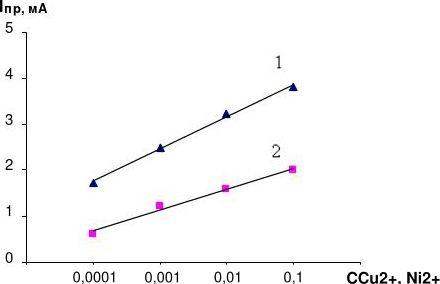
\includegraphics[width=0.5\textwidth]{image44}
\caption*{Figure 1 - Dependence of the limiting reduction current of
Cu\textsuperscript{2+}(1) and Ni\textsuperscript{2+}(2) on a copper
electrode on the concentration of ions in solution. Ion concentrations,
mol/l: 0,0001; 0,001; 0,01; 0,1}
\end{figure}

\begin{multicols}{2}
The reduction of copper, nickel and zinc on a titanium electrode occurs
in a more negative potential range compared to copper (Table 2),
although the nature of the electrode does not significantly affect the
shape of the polarograms. The value of the half-wave potential on a
titanium electrode shifts to a less negative region with an increase in
the concentration of ions in the solution, whereas on a copper electrode
it remains at the same level. So, for example, when the copper
concentration changes from 10\textsuperscript{-4} to
10\textsuperscript{-1} M on a titanium electrode, the half-wave
potential changes from -0,68 V to -0,54 V, on a copper electrode it
remains at -0,54 V to -0,52 V.
\end{multicols}

\begin{figure}[H]
    \centering
    \begin{subfigure}[b]{0.45\textwidth}
        \centering
        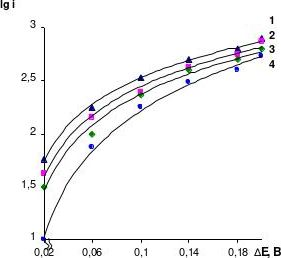
\includegraphics[width=\textwidth]{image45}
        \caption*{Figure 2 - Dependence of lg I on the ΔE-reduction process of
        Cu\textsuperscript{2+} concentration of 10\textsuperscript{-1} mol/l on
        a titanium electrode with the addition of citric acid, g-eq/l: 1-0,01;
        2-0,025; 3-0,05; 4-0,1}
    \end{subfigure}
    \hfill
    \begin{subfigure}[b]{0.45\textwidth}
        \centering
        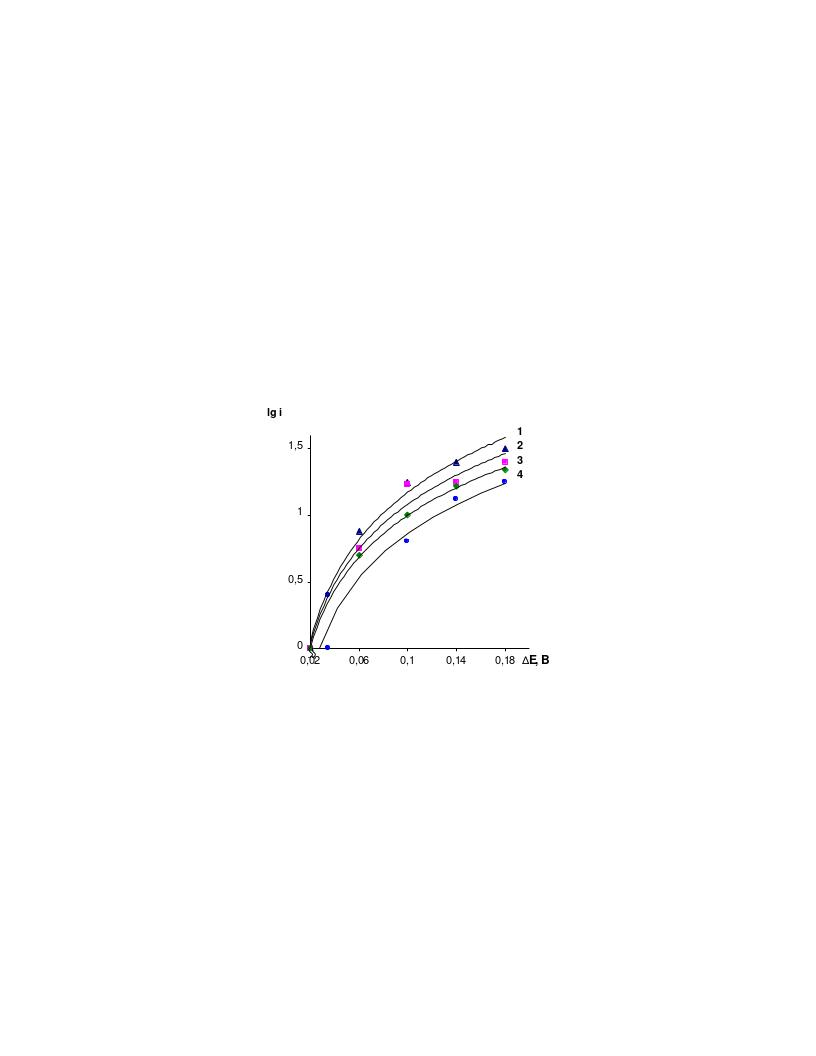
\includegraphics[width=\textwidth]{image46}
        \caption*{Figure 3. Dependence of lg I on the ΔE-reduction process of
        Ni\textsuperscript{2+} concentration of 10\textsuperscript{-1} mol/l on
        a copper electrode with the addition of citric acid, g-eq/l: 1-0,01;
        2-0,025; 3-0,05; 4-0,1}
    \end{subfigure}
    \begin{subfigure}[b]{0.45\textwidth}
        \centering
        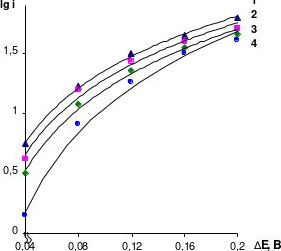
\includegraphics[width=\textwidth]{image47}
        \caption*{Figure 4 - Dependence of lg I on the ΔE-reduction process of
        Zn\textsuperscript{2+} concentration of 10\textsuperscript{-1} mol/l on
        a copper electrode with the addition of citric acid, g-eq/l: 1-0,01;
        2-0,025; 3-0,05; 4-0,1}
    \end{subfigure}
\end{figure}

\begin{longtable}[]{@{}
  >{\raggedright\arraybackslash}p{(\columnwidth - 10\tabcolsep) * \real{0.1310}}
  >{\raggedright\arraybackslash}p{(\columnwidth - 10\tabcolsep) * \real{0.1262}}
  >{\raggedright\arraybackslash}p{(\columnwidth - 10\tabcolsep) * \real{0.1359}}
  >{\raggedright\arraybackslash}p{(\columnwidth - 10\tabcolsep) * \real{0.1497}}
  >{\raggedright\arraybackslash}p{(\columnwidth - 10\tabcolsep) * \real{0.1497}}
  >{\raggedright\arraybackslash}p{(\columnwidth - 10\tabcolsep) * \real{0.3075}}@{}}
\caption*{Table 2 - The effect of the concentration of ammonia complexes on -E1/2
and I\textsubscript{pr}} \\
\toprule\noalign{}
\multicolumn{3}{c}{Concentration, mol/l} &
\multirow{2}{*}{\begin{minipage}[b]{\linewidth}\raggedright
I\textsubscript{pr}, мA
\end{minipage}} &
\multirow{2}{*}{\begin{minipage}[b]{\linewidth}\raggedright
-Е\textsubscript{1/2}, В
\end{minipage}} &
\multirow{2}{*}{\begin{minipage}[b]{\linewidth}\raggedright
Cathode material
\end{minipage}} \\
\begin{minipage}[b]{\linewidth}\raggedright
Cu\textsuperscript{2+}
\end{minipage} & \begin{minipage}[b]{\linewidth}\raggedright
Ni\textsuperscript{2+}
\end{minipage} & \begin{minipage}[b]{\linewidth}\raggedright
Zn\textsuperscript{2+}
\end{minipage} \\
\midrule\noalign{}
\endhead
\bottomrule\noalign{}
\endlastfoot
10\textsuperscript{-1} & & & 3,9 & 0,52 & \multirow{4}{*}{Cu} \\
10\textsuperscript{-2} & & & 3,15 & 0,54 \\
10\textsuperscript{-3} & & & 2,4 & 0,53 \\
10\textsuperscript{-4} & & & 1,7 & 0,54 \\
\hline
& 10\textsuperscript{-1} & & 3,3 & 0,58 & \multirow{4}{*}{Cu} \\
& 10\textsuperscript{-2} & & 2,85 & 0,60 \\
& 10\textsuperscript{-3} & & 2,3 & 0,59 \\
& 10\textsuperscript{-4} & & 1,8 & 0,56 \\
\hline
& & 10\textsuperscript{-1} & 2 & 0,62 & \multirow{4}{*}{Cu} \\
& & 10\textsuperscript{-2} & 1,5 & 0,58 \\
& & 10\textsuperscript{-3} & 1,2 & 0,58 \\
& & 10\textsuperscript{-4} & 0,7 & 0,565 \\
\hline
10\textsuperscript{-1} & & & 60 & 0,54 & \multirow{4}{*}{Ti} \\
10\textsuperscript{-2} & & & 47 & 0,60 \\
10\textsuperscript{-3} & & & 35 & 0,63 \\
10\textsuperscript{-4} & & & 22 & 0,66 \\
\hline
& 10\textsuperscript{-1} & & 51 & 0,62 & \multirow{4}{*}{Ti} \\
& 10\textsuperscript{-2} & & 40 & 0,64 \\
& 10\textsuperscript{-3} & & 29 & 0,63 \\
& 10\textsuperscript{-4} & & 18 & 0,65 \\
\hline
& & 10\textsuperscript{-1} & 44 & 0,68 & \multirow{4}{*}{Ti} \\
& & 10\textsuperscript{-2} & 34 & 0,67 \\
& & 10\textsuperscript{-3} & 25 & 0,64 \\
& & 10\textsuperscript{-4} & 15 & 0,635 \\
\end{longtable}

\begin{multicols}{2}
Citric acid shifts the copper half-wave potential to a more negative
area. If, in the absence of citric acid, the difference in the half-wave
potentials of copper and nickel is (on a titanium electrode) -0,08 V,
copper and zinc - 0,14 V, then in the presence of citric acid in the
solution, the difference in the half-wave potentials of copper and
nickel is 0,015 V, copper and zinc -0,005 V. In this case, the reduction
potentials of copper, nickel and zinc converge. This promotes the joint
electrodeposition of Cu, Ni and Zn. Table 3 shows the data on the effect
of citrate ions on the reduction potentials and the magnitude of the
limiting current.
\end{multicols}

\begin{longtable}[]{@{}
  >{\raggedright\arraybackslash}p{(\columnwidth - 12\tabcolsep) * \real{0.1422}}
  >{\raggedright\arraybackslash}p{(\columnwidth - 12\tabcolsep) * \real{0.1404}}
  >{\raggedright\arraybackslash}p{(\columnwidth - 12\tabcolsep) * \real{0.1310}}
  >{\raggedright\arraybackslash}p{(\columnwidth - 12\tabcolsep) * \real{0.1479}}
  >{\raggedright\arraybackslash}p{(\columnwidth - 12\tabcolsep) * \real{0.1381}}
  >{\raggedright\arraybackslash}p{(\columnwidth - 12\tabcolsep) * \real{0.1422}}
  >{\raggedright\arraybackslash}p{(\columnwidth - 12\tabcolsep) * \real{0.1582}}@{}}
\caption*{Table 3 -The effect of citric acid additions on -E\textsubscript{1/2}
and Ipr} \\
\toprule\noalign{}
\multicolumn{3}{c}{Concentration, mol/l} &
\multirow{2}{*}{\begin{minipage}[b]{\linewidth}\raggedright
C\textsubscript{citric acid}
\end{minipage}} &
\multirow{2}{*}{\begin{minipage}[b]{\linewidth}\raggedright
I\textsubscript{pr}, мA
\end{minipage}} &
\multirow{2}{*}{\begin{minipage}[b]{\linewidth}\raggedright
-Е\textsubscript{1/2}, В
\end{minipage}} &
\multirow{2}{*}{\begin{minipage}[b]{\linewidth}\raggedright
Cathode material
\end{minipage}} \\
\begin{minipage}[b]{\linewidth}\raggedright
Cu\textsuperscript{2+}
\end{minipage} & \begin{minipage}[b]{\linewidth}\raggedright
Ni\textsuperscript{2+}
\end{minipage} & \begin{minipage}[b]{\linewidth}\raggedright
Zn\textsuperscript{2+}
\end{minipage} \\
\midrule\noalign{}
\endhead
\bottomrule\noalign{}
\endlastfoot
10\textsuperscript{-1} & & & 0 & 3,9 & 0,52 & \multirow{5}{*}{Cu} \\
& & & 0,01 & 3,5 & 0,54 \\
& & & 0,025 & 3,2 & 0,53 \\
& & & 0,05 & 3,4 & 0,54 \\
& & & 0,1 & 3,9 & \\
\hline
& 10\textsuperscript{-1} & & 0 & 3,3 & 0,58 & \multirow{5}{*}{Cu} \\
& & & 0,01 & 2,6 & 0,60 \\
& & & 0,025 & 2,1 & 0,59 \\
& & & 0,05 & 1,6 & 0,56 \\
& & & 0,1 & 1,5 & \\
\hline
& & 10\textsuperscript{-1} & 0 & 2 & 0,62 & \multirow{5}{*}{Cu} \\
& & & 0,01 & 1,7 & 0,58 \\
& & & 0,025 & 1,5 & 0,58 \\
& & & 0,05 & 1,6 & 0,565 \\
& & & 0,1 & 1,3 & \\
\hline
10\textsuperscript{-1} & & & 0 & 60 & 0,54 & \multirow{5}{*}{Ti} \\
& & & 0,01 & 58 & 0,60 \\
& & & 0,025 & 56 & 0,63 \\
& & & 0,05 & 50 & 0,66 \\
& & & 0,1 & 40 & \\
\hline
& 10\textsuperscript{-1} & & 0 & 51 & 0,62 & \multirow{5}{*}{Ti} \\
& & & 0,01 & 48 & 0,64 \\
& & & 0,025 & 41 & 0,63 \\
& & & 0,05 & 41 & 0,65 \\
& & & 0,1 & 36,6 & \\
\hline
& & 10\textsuperscript{-1} & 0 & 44 & 0,68 & \multirow{5}{*}{Ti} \\
& & & 0,01 & 41 & 0,67 \\
& & & 0,025 & 38 & 0,64 \\
& & & 0,05 & 37 & 0,635 \\
& & & 0,1 & 32 & \\
\end{longtable}

\begin{multicols}{2}
The value of the limiting current decreased with an increase in the
concentration of the citric acid additive, especially when using a
titanium electrode. Glycine additives shift the half-wave potential of
both copper, nickel and zinc to a less negative region (by 0,078 V for
copper, 0,11 V for nickel, 0,12 V for zinc). But a significant gap
between them remains. The presence of glycine also led to a significant
change in the value of the limiting current at the electrodes (Table 4).

Changes in the voltammetric behavior of metals in the presence of citric
and aminoacetic (glycine) acids are associated with the noted processes
of complexation, the transition of metals from one complex form to
another.
\end{multicols}

\begin{longtable}[]{@{}
  >{\raggedright\arraybackslash}p{(\columnwidth - 12\tabcolsep) * \real{0.1365}}
  >{\raggedright\arraybackslash}p{(\columnwidth - 12\tabcolsep) * \real{0.1346}}
  >{\raggedright\arraybackslash}p{(\columnwidth - 12\tabcolsep) * \real{0.1273}}
  >{\raggedright\arraybackslash}p{(\columnwidth - 12\tabcolsep) * \real{0.1407}}
  >{\raggedright\arraybackslash}p{(\columnwidth - 12\tabcolsep) * \real{0.1330}}
  >{\raggedright\arraybackslash}p{(\columnwidth - 12\tabcolsep) * \real{0.1379}}
  >{\raggedright\arraybackslash}p{(\columnwidth - 12\tabcolsep) * \real{0.1899}}@{}}
\caption*{Table 4 - The effect of glycine additives on -E\textsubscript{1/2} and Ipr} \\
\toprule\noalign{}
\multicolumn{3}{c}{Concentration, mol/l} &
\multirow{2}{*}{\begin{minipage}[b]{\linewidth}\raggedright
Glycine\textsubscript{, г-экв/л}
\end{minipage}} &
\multirow{2}{*}{\begin{minipage}[b]{\linewidth}\raggedright
I\textsubscript{пр}, мA
\end{minipage}} &
\multirow{2}{*}{\begin{minipage}[b]{\linewidth}\raggedright
-Е\textsubscript{1/2}, В
\end{minipage}} &
\multirow{2}{*}{\begin{minipage}[b]{\linewidth}\raggedright
Cathode material
\end{minipage}} \\
\begin{minipage}[b]{\linewidth}\raggedright
Cu\textsuperscript{2+}
\end{minipage} & \begin{minipage}[b]{\linewidth}\raggedright
Ni\textsuperscript{2+}
\end{minipage} & \begin{minipage}[b]{\linewidth}\raggedright
Zn\textsuperscript{2+}.
\end{minipage} \\
\midrule\noalign{}
\endhead
\bottomrule\noalign{}
\endlastfoot
10\textsuperscript{-1} & & & 0 & 3,9 & 0,52 & \multirow{5}{*}{Cu} \\
& & & 0,01 & 3,4 & 0,54 \\
& & & 0,025 & 3,1 & 0,53 \\
& & & 0,05 & 3,3 & 0,54 \\
& & & 0,1 & 3,1 & \\
\hline
& 10\textsuperscript{-1} & & 0 & 3,3 & 0,58 & \multirow{5}{*}{Cu} \\
& & & 0,01 & 2,9 & 0,60 \\
& & & 0,025 & 2,5 & 0,59 \\
& & & 0,05 & 2,6 & 0,56 \\
& & & 0,1 & 2,65 & \\
\hline
& & 10\textsuperscript{-1} & 0 & 2 & 0,62 & \multirow{5}{*}{Cu} \\
& & & 0,01 & 1,7 & 0,54 \\
& & & 0,025 & 1,6 & 0,52 \\
& & & 0,05 & 1,8 & 0,525 \\
& & & 0,1 & 1,5 & 0,50 \\
\end{longtable}

\begin{multicols}{2}
{\bfseries Conclusions.} Thus, if complexing reagents - ammonia, citric
acid, glycine - are introduced into the system, sufficiently stable
complexes with Cu\textsuperscript{2+}, Ni\textsuperscript{2+},
Zn\textsuperscript{2+} ions are formed in the solution. Glycine makes
the system more stable, which is associated with the formation of
homogeneous complexes. Citric acid reduces the limiting current, but the
equilibrium character remains unchanged. At the same time, the reduction
potentials of copper, nickel and zinc converge, which contributes to
their joint electrodeposition. The results of the research can be used
to solve problems in the field of processing solutions derived from the
cycle of electrolytic refining of copper.
\end{multicols}

\begin{center}
{\bfseries Литература}
\end{center}

\begin{enumerate}
\item
Омаров Х.Б., Жарменов А.А., Сагиндыкова З.Б. Мышьяк в гидрохимических
процессах медного производства. - Караганда: Изд-во КарГУ, 2007. - 167
с.

\item
Жарменов А.А., Милицин В.В., Омаров Х.Б. и др. Опытно-промышленные
испытания аммиачной технологии переработки медного электролита на АО
«Жезказганцветмет» // Промышленность Казахстана. 2000. - №3.- С. 51-93.

\item
Cumbal L. Sen Gupta A.K. Arsenic removal using polymer-supported
hydrated lron (III) oxide nanoparticles: role of donnan membrane effect
// Environ. Sci. Technol. - 2005, №39. - P. 6508-6515.

\item
Шаталов В.В., Смирнова Н.М., Глухова Л.П., Савельева Т.И. Мембранные
процессы в гидрометаллургии // Цветные металлы. - 2003. - №4. - С.
53-57.

\item
Тодоров С.А., Лайнер Ю.А., Медведев А.С. Утилизация
низкоконцентрированных растворов с использованием электродиализа //
Цветная металлургия. - 2004. - №3. - С. 37-39.

\item
Шапошник В.А., Котов В.,В, Кобелева Н.С. Влияние плотности тока на
эффективность разделения ионов при электродиализе // Прикладная химия.
- 1980. - №5. - С. 1058-1061.

\item
Разделение и очистка веществ методом электродиализа с ионообменными
мембранами // РЖХ. - 1986. - 5Л3Б.

\item
Певницкая М.В., Гнусин Н.П., Лаврова Т.А. Электрический перенос ионов
через катионитовую мембрану в смешанных растворах солей // Известия СO
АН CССР, Серия химических наук. - 1965. - №7. - С. 13-18.

\item
Жарменов А.А. Электродиализная переработка растворов
электролитического рафинирования меди: автореф\ldots{} канд. техн. наук:
- Алма-Ата, 1982. -21с.

\item
Жарменов А.А., Шарипов М.Ш. Избирательность катионитовых мембран в
сернокислых растворах никеля и меди //Прикладная химия. - 1985.
-№2.-С.275-278.

\item
Agraz R., Sevilla M.T. and Hernandez L. Chemically modified
electrode for the simultaneous determination of trace metals and
speciation analysis. Anal. Chim. Acta. 1993. Vol. 273. P. 205.

\item
Багхери А., Маранд М.Х. Вольтамперометрическое и потенциометрическое
определение Cu\textsuperscript{2+} с помощью электрохимического сенсора
на основе сверхокисленного полипиррола. Электрохимия. 2020. Т. 56. № 6.
С. 483-493.

\item
Касач А.А., Харитонов Д.С., Радченко С.Л. и др. Исследование влияния
параметров импульсного электролиза на процесс электроосаждения сплава
медь-олово из сульфатного электролита. Электрохимия. 2020. Т. 56. №9.
С.820-830.

\item
Zanganeh A.R. and Amini M.K. Polypyrrole-modified electrodes with
induced recognition sites for potentiometric and voltammetric detection
of copper (II) ion. Sens. Act. B. 2008/ Vol. 135. P. 358.

\item
Meudre C., Ricg I., Hihn J.Y. and others. Absorption of gelatin
during electrodeposition of copper and tin-copper alloys from acid
sulfate electrolyte. Surf. Coat. Tech., 2014. Vol. 252. P.93.

\item
Желис Х.П. Винкавичус И.И. Химическое осаждение никелевых сплавов //
Труды АН Лит ССР. -1985 Б. - № 61.151. - С.3-9.

\item
А.С. 1148903 СССР. Способ переработки медного электролита
электролизом / А.А. Жарменов и др.; опубл. 1985, Бюл. №13.
\end{enumerate}

\begin{center}
{\bfseries References}
\end{center}

\begin{enumerate}
\item
Omarov Kh.B., Zharmenov A.A., Sagyndykova Z.B. Myshyak v
gidrochemitheskikh processakh mednogo proizvodstva. -Karaganda:Izd-vo
KarGU, 2007. -167s.

\item
Zharmenov A.A., Milicin V.V., Omarov Kh.B. i dr. Opytno-promyshlennye
ispytania ammiathnoi technologii pererabotki mednogo electrolita na AO
«Zhezkazgancvetmet» // Promyshlennost Kazakhstana. 2000. -№3. -S. 51-93.

\item
Cumbal L. Sen Gupta A.K. Arsenic removal using polymer-supported
hydrated lron (III) oxide nanoparticles: role of donnan membrane effect
// Environ. Sci. Technol. - 2005, №39. - P. 6508-6515.

\item
Shatalov V.V., Smirnova N.M., Glukhova L.P., Savelieva T.I.
Membrannye process v gidrometallurgii // Cvetnye metally. - 2003. -№3.
-S. 53-57.

\item
Todorov S.A., Lainer Ua.A., Medvedev A.S. Utilizaciya
nizkoconcenrirovannykh rastvorov s ispolzovaniem electrodializa //
Cvetnaya metallurgiya. - 2004. - №3. -S. 37-39.

\item
Shaposhnik V.A., Kotov V.V., Kobeleva N.S. Vliyanie plotnosti toka na
effectibnost razdeleniya ionov pri electrodialize // Pricladnaya
chimiya. - 1980. - №5. - S. 1058-1061.

\item
Razdelenie i othistka veschestv metodom electrodializa s
ionoobmennymi membranami // RZhCh. - 1986. - 5L3B.

\item
Pevnickaya M.V., Gnusin N.P., Lavrova T.A. Electritheskii perenos
ionov therez kationitovuua membranu v smeshannych rastvorach solei //
Izvestiya SO AN SSSR, Seriya chimitheskich nauk. - 1965. - №7. - S.
13-18.

\item
Zharmenov A.A. Electrodializnaya pererabotka rastvorov
electrolititheskogo rafinirovaniya medi: avtoref\ldots kand. techn.
nauk: - Alma-Ata, 1982. -21s.

\item
Zharmenov A.A., Sharipov M.Sh. Izbiratelnost kationitovych membran v
sernokislych rastvorach nicelya i medi // Pricladnaya chimiya. . -
1985. -№2.-S.275-278.

\item
Agraz R., Sevilla M.T. and Hernandez L. Chemically modified
electrode for the simultaneous determination of trace metals and
speciation analysis. Anal. Chim. Acta. 1993. Vol. 273. P. 205.

\item
Bagcheri A., Marand M.Ch. Voltamperometritheskoe i
potenciometritheskoe opredelenie Cu\textsuperscript{2+} s pomoschua
electrochimitheskogo sensora na osnove sverchokislennogo polipirolla.
Electochimiya. 2020. Т. 56. № 6. S. 483-493.

\item
Kasath A.A., Charitonov D.S., Radthenko S.L. i dr. Issledovanie
vliyaniya parametrov impulsnogo electroliza na process electroosagdeniya
splava med-olovo iz sulfatnogo electrolita. Electochimiya. 2020. Т. 56.
№9. S.820-830.

\item
Zanganeh A.R. and Amini M.K. Polypyrrole-modified electrodes with
induced recognition sites for potentiometric and voltammetric detection
of copper (II) ion. Sens. Act. B. 2008/ Vol. 135. P. 358.

\item
Meudre C., Ricg I., Hihn J.Y. and others. Absorption of gelatin
during electrodeposition of copper and tin-copper alloys from acid
sulfate electrolyte. Surf. Coat. Tech., 2014. Vol. 252. P.93.

\item
Zhelis Ch.P., Vinkavithus I.I. Chimicheskoe osazhdenie nicelevych
splavov // Trudy AN Lit. SSR. -1985 B. - № 61.151. - S.3-9.

\item
A.S. 1148903 SSSR. Sposob pererabotki mednogo electrolita
electrolizom / A.A.Zharmenov i dr.; opubl. 1985, Bual. №13.
\end{enumerate}

\emph{{\bfseries Information about authors}}

\begin{itemize}
\item
Omarov Khylysh Beisenovich, Doctor of Technical Sciences, Professor,
Professor of the Department of Chemistry, Chemical Technology and
Ecology, Kazakh University of Technology and Business, Republic of
Kazakhstan, Astana, e-mail:
homarov1963@mail.ru

\item
Nurtai Zhadyra Tastenbekovna, PhD, Associate Professor of the Department
of Chemistry, Chemical Technology and Ecology, Kazakh University of
Technology and Business, Republic of Kazakhstan, Astana, e-mail:
zhadira\_nurtai@mail.ru

\item
Kopylov Nikolai Ivanovich, Doctor of Technical Sciences, Professor,
Leading Researcher, Institute of Solid State Chemistry and
Mechanochemistry, Siberian Branch of the Russian Academy of Sciences,
Russia, Novosibirsk, e-mail:
kopylov@narod.ru
\end{itemize}

\emph{{\bfseries Сведения об авторах}}

\begin{itemize}
\item
Омаров Хылыш Бейсенович, доктор технических наук, профессор, профессор
кафедры химии, химической технологии и экологии Казахского университета
технологии и бизнеса, Республика Казахстан, г. Астана, e-mail:
homarov1963@mail.ru

\item
Нұртай Жадыра Тастенбековна, доктор PhD, ассоциированный профессор
кафедры химии, химической технологии и экологии Казахского университета
технологии и бизнеса, Республика Казахстан, г. Астана, e-mail:
zhadira\_nurtai@mail.ru

\item
Копылов Николай Иванович, доктор технических наук, профессор, ведущий
научный сотрудник Института химии твердого тела и механохимии Сибирского
отделения Российской Академии наук, Россия, г. Новосибирск, e-mail:
kopylov@narod.ru
\end{itemize}
